\documentclass[utf8]{ctexart}
\usepackage[margin=1in]{geometry}
\usepackage{setspace}
\usepackage{hyperref}
\usepackage{graphicx}
\usepackage{booktabs}
\usepackage{longtable}
\usepackage{amsmath}
\usepackage{tikz}
\usetikzlibrary{arrows.meta,positioning,shapes.geometric}
\usepackage{float}
\usepackage{caption}
\usepackage{verbatim}

\title{课程项目技术报告：横版格斗游戏中的关键软件技术}
\author{
姓名：李子嘉 \\
学号：2024012325 \\
邮箱：zj-li24@mails.tsinghua.edu.cn \\
电话：(+86) 13585915409
}
\date{\today}

\begin{document}
\maketitle
\tableofcontents
\newpage

\section*{摘要}
\addcontentsline{toc}{section}{摘要}

本报告围绕题目 3.19（横版格斗对战游戏）的工程实践，提炼出六项在项目中起到关键作用的软件技术。这些技术并非预先选定的"展示项目"，而是从游戏的实际需求出发推导出的必需品——一个模块复杂、交互密集的格斗游戏天然要求这些技术作为支撑。每项技术按照"游戏需求引出的问题 → 为什么简单方案不够 → 技术方案与设计思路 → 代码验证 → 替代方案分析"的结构展开。六项技术分别为：面向对象技术在游戏系统中的应用、事件驱动的模块间松耦合通信、数据驱动的玩法可扩展性、有限状态机驱动的NPC决策、实时游戏主循环的时序设计、以及跨平台构建系统的抽象与配置。

\newpage

% ============================================================
%  游戏概览（帮助理解后续技术讨论的上下文）
% ============================================================
\section{游戏概览}

在进入技术分析之前，本节从玩家视角介绍游戏的实际面貌，为后续各技术模块提供上下文。如果评阅者只读各技术章节而不了解游戏本身，将难以判断技术方案的合理性。

\subsection{游戏是什么}

本项目是一个基于 Qt 图形界面的横版格斗对战游戏。两名角色在 2D 平台上进行对战——通过键盘操控角色移动、跳跃、攻击、切换武器和释放法术，目标是击败对手（将对方生命值削减至零）。

游戏支持三种模式：

\begin{itemize}
  \item \textbf{人机对战（AI）}：玩家操控 P1，P2 由 AI 控制。适合单人快速体验。
  \item \textbf{双人对战（PVP）}：两名玩家使用同一键盘的不同键位分别操控 P1 和 P2。P1 键位为 WASD（移动）+ F（攻击）+ G/C（切换武器/法术），P2 键位为 IJKL（移动）+ O（攻击）+ N/U（切换武器/法术）。
  \item \textbf{无尽模式（ENDLESS）}：玩家操控 P1 连续对抗多轮 AI 对手（P2）。每轮结束后玩家从三个随机词条中选择一个增益，对手的伤害输出也会逐轮递增。一方阵亡即该轮结束——若玩家阵亡则游戏终止并显示该轮的结算统计（总伤害、击杀数、生存时间）；若 AI 阵亡则进入下一轮。玩家死亡判定生命值归零即死；AI 死亡判定生命值归零 + 1 秒后解除 immortal 保护才会死。无尽模式下 AI 拥有 \texttt{endlessImmortal} 属性以延长存活时间到保护期结束。这个模式的压力来自于对手伤害的递增曲线——随着轮数增加，容错率下降，迫使玩家在词条选择和打法上做取舍。
\end{itemize}

\subsection{玩家能做什么}

玩家在一局游戏中可执行以下操作：

\begin{itemize}
  \item \textbf{移动}：左右移动与跳跃（P1：A/D + W/空格；P2：J/L + I），受平台物理和重力约束。
  \item \textbf{近战攻击}：拳击（默认武器，无弹药限制）和小刀（伤害更高），需要贴近对手。
  \item \textbf{远程攻击}：投掷实心球（抛物线弹道，有弹药限制）、步枪射击（直线弹道，5 发弹匣）、狙击枪射击（直线弹道，2 发弹匣，伤害最高），各有独立的弹药计数和伤害倍率。
  \item \textbf{切换武器槽}：C/N 键在已持有的武器间循环切换，拾取新武器时自动加入槽位。
  \item \textbf{释放法术}：Q/U 键释放所选法术，包括定身术（冻结对手）、隐身术（脱离视野，脱离后有破影一击）、铜头铁臂（弹反近战伤害）、安身法（屏障内减伤和回血）、身外身法（召唤克隆体）和禁字法（放弃法术换伤害加成）。
  \item \textbf{拾取掉落物}：地面上定时刷新或击败敌人后掉落的武器、词条卡片和血瓶，走近自动拾取。
\end{itemize}

\subsection{对局流程（从启动到结算）}

启动程序后进入主菜单，点击"开始"进入设置页面。设置页面中，玩家可以选择：
\begin{itemize}
  \item 游戏模式（人机 / 双人 / 无尽）
  \item 场景（默认或草地——草地场景中不移动时自动蹲下，增加策略纵深）
  \item 血量上限、弹药数量等数值参数（或使用预设档位）
  \item P1 和 P2 各选一个法术（或随机）
\end{itemize}

点击"开始对局"后进入游戏主界面。60FPS 的帧循环即刻启动。对局中，画面左侧实时显示双方血条、武器图标、词条摘要和法术冷却进度。无尽模式下，每轮结束弹出三选一词条面板，选择后立刻生效。

一方阵亡后，对局结束。单局模式下显示胜负画面，玩家按任意键返回主菜单。无尽模式下显示结算面板，包含总伤害、击杀数、生存时间和排行榜，玩家可选择"再来一局"或"返回菜单"。

\subsection{系统构成概览}

从技术角度看，这个格斗游戏背后是 10+ 个模块的协同工作：

\begin{itemize}
  \item \textbf{Player}：管理角色的生命值、武器槽、词条集合、法术状态和动画
  \item \textbf{PlayerController}：将玩家输入（或 AI 指令）转换为角色动作，管理攻击冷却、受击硬直和地图碰撞修正
  \item \textbf{Entity / Ball / Bullet / DropItem}：所有飞行物和掉落物的运动、碰撞与生命周期，通过多态统一管理
  \item \textbf{CombatManager}：统一结算所有碰撞事件（近战互殴、投掷物命中、子弹命中），计算伤害并应用硬直/击退/状态
  \item \textbf{GameAI}：NPC 的决策层，基于 FSM 和人格系统生成移动与攻击意图
  \item \textbf{Map}：管理场景碰撞体（平台、地面、墙壁），提供平台间 BFS 寻路服务
  \item \textbf{SoundManager}：单例模式的全局音效加载与播放
  \item \textbf{Widget（游戏主界面）}：驱动每帧更新循环，统筹所有模块的执行顺序，渲染画面和 UI
  \item \textbf{EndlessRecordManager}：记录无尽模式每轮的伤害和击杀统计
  \item \textbf{SetupWidget / MainWindow}：对局设置界面和主窗口页面导航框架
  \item \textbf{EndlessResultWidget / ModifierOverlay}：无尽模式结算面板和词条选择弹窗
\end{itemize}

正是这个模块规模和多对多的交互关系，使得后续讨论的每一项技术都有了存在的必要性——如果只有两三个模块，这些技术方案就是过度设计。

\newpage

% ============================================================
%  技术 1：面向对象技术在游戏系统中的应用
% ============================================================
\section{技术一：面向对象技术在游戏系统中的应用}

\subsection{游戏中引出的问题}

一个横版格斗游戏存在多种可交互对象：玩家角色、AI对手、实心球（投掷物）、步枪子弹、狙击枪子弹、掉落物（武器/血瓶/词条）。尽管这些对象的行为差异巨大——子弹直线飞行、实心球受重力走抛物线、掉落物静止不动、玩家角色有复杂动画——它们共享一组基本需求：

\begin{enumerate}
  \item 每帧都要更新位置（update）
  \item 每帧都要绘制到屏幕（draw）
  \item 需要提供碰撞箱供战斗系统判定（hitbox）
  \item 需要知道自己何时该被销毁（shouldBeRemoved）
  \item 与玩家发生碰撞时触发特定行为（onCollideWithPlayer）
  \item 需要暴露伤害值和武器类型供伤害计算（getDamage、getWeaponType）
\end{enumerate}

假设不用面向对象技术，最直接的替代方案是为每种对象类型写一套独立的处理逻辑——每个游戏帧里，函数 A 处理球的运动，函数 B 处理子弹的运动，函数 C 处理掉落物的计时，函数 D 挨个绘制所有东西。这意味着：每增加一种新实体类型，就要在游戏循环的每个环节追加新的分支。本项目目前只有 4 种实体（球、步枪子弹、狙击子弹、掉落物），但如果按上述"每类一套逻辑"的做法，游戏循环中已经需要写 4 套相似却不完全相同的处理路径；扩展到 10 种实体时，维护成本将按 实体类型数 $\times$ 处理环节数 增长。这正是本项目采用继承体系要避免的局面。

\subsection{技术方案与设计思路}

本项目的核心思路是：\textbf{用一个抽象基类 \texttt{Entity} 定义"所有可交互对象"的统一接口，每个具体实体类型实现自己的行为}。关键设计决策如下。

\subsubsection{Entity 基类：定义最小接口}

\texttt{entity.h} 中定义的基类只包含所有实体共有的数据和纯虚函数接口（参见文件 \texttt{entity.h}）：

\begin{itemize}
  \item \textbf{共有的数据}：位置（\texttt{position}）、速度（\texttt{velocity}）、重力常量、阻力常量、帧时间 \texttt{dt}、所属者 ID（\texttt{parentId}）、层级（\texttt{layer}）等。这些是任何运动物体都需要的物理属性。
  \item \textbf{纯虚函数接口}：\texttt{update()}、\texttt{draw()}、\texttt{hitbox()}、\texttt{getDamage()}、\texttt{getWeaponType()}、\texttt{onCollideWithPlayer()}、\texttt{shouldBeRemoved()}。每个具体子类\textbf{必须}实现这些函数。
  \item \textbf{已实现的通用方法}：\texttt{applyGravity()}（施加重力加速度）、\texttt{stop()}（施加阻力减速）、\texttt{getPos()}（返回当前位置）、\texttt{getDir()}（根据速度方向返回朝向）。这些方法的行为对所有实体一致，放在基类中避免代码重复。
\end{itemize}

\begin{verbatim}
class Entity
{
public:
    Entity(QPointF pos, int id=0, float frozenBonus = 1.0f);
    virtual void update() = 0;
    virtual void draw(QPainter& painter) = 0;
    virtual void onCollideWithPlayer(){};
    virtual float getDamage(int id){return 0;};
    virtual QRect hitbox(){};
    virtual Player::WeaponType getWeaponType(){ return Player::WeaponType::punch; };
    virtual bool shouldBeRemoved(){};
    void applyGravity();
    void stop();
    // ...
protected:
    QPointF position;
    QPointF velocity;
    float dt;
    int parentId;
    int layer;
};
\end{verbatim}

\subsubsection{三个典型子类，三种不同的行为实现}

\textbf{Ball（实心球）}继承 Entity，在虚函数中实现了：
\begin{itemize}
  \item \texttt{update()}：根据速度和重力更新位置，递减生命周期计时器，到期后标记删除。
  \item \texttt{getDamage()}：基于动能公式（初速度和质量）计算撞击伤害，并受 frozenBonus 的定身增伤加成。
  \item \texttt{onCollideWithPlayer()}：碰撞后直接标记为待删除（球击中目标即消失）。
  \item \texttt{getWeaponType()}：返回 \texttt{ball}。
\end{itemize}

\textbf{Bullet（子弹）}继承 Entity，行为与 Ball 明显不同：
\begin{itemize}
  \item \texttt{update()}：仅有水平匀速运动（无重力），靠设定初速度 $v_x$ 直线飞行。
  \item \texttt{getDamage()}：伤害基于发射者的基础攻击力乘以武器倍率，而非动能公式。
  \item \texttt{getWeaponType()}：根据内部 type 字段（1 = rifle, 2 = sniper）返回不同武器类型。
  \item 步枪子弹和狙击子弹共用同一个 \texttt{Bullet} 类，通过构造函数参数 \texttt{type} 区分行为。
\end{itemize}

\textbf{DropItem（掉落物）}继承 Entity，行为最简单：
\begin{itemize}
  \item \texttt{update()}：仅递减存活计时器，不移动（位置固定）。
  \item \texttt{shouldBeRemoved()}：在超时或被玩家拾取后返回 true。
  \item \texttt{getDamage()}：返回 0（掉落物不会造成伤害）。
  \item 额外提供 \texttt{isCollectedBy(Player*)} 方法判断是否被玩家拾取。
\end{itemize}

\subsubsection{多态在游戏循环中的实际使用}

在多处关键路径中，代码通过 \texttt{Entity*} 基类指针操作具体对象，完全不需要知道运行时类型：

\textbf{场景一：统一渲染}（\texttt{widget.cpp}）——所有实体通过同一段代码绘制：
\begin{verbatim}
for (const auto& entity : entities) {
    if (entity) {
        entity->draw(painter);   // 虚函数调用，每个子类画自己
    }
}
\end{verbatim}

\textbf{场景二：统一清理过期对象}（\texttt{widget.cpp}）——用 \texttt{remove\_if} 配合虚函数判断：
\begin{verbatim}
entities.erase(std::remove_if(entities.begin(), entities.end(),
                   [](const std::shared_ptr<Entity>& e) {
                       return e->shouldBeRemoved();  // 每个子类自己决定何时过期
                   }), entities.end());
\end{verbatim}

\textbf{场景三：战斗碰撞结算}（\texttt{combatmanager.cpp}）——战斗管理器只知道自己面对的是 \texttt{Entity*}，通过虚函数获取决策所需信息：
\begin{verbatim}
void CombatManager::checkEntityVsPlayerCollision(Entity *e, PlayerController *p) {
    const auto weaponType = e->getWeaponType();  // 虚函数
    float rawDmg = e->getDamage(p->getId());      // 虚函数，球和子弹计算方式完全不同
    float defMult = p->getDefenseMultiplier(e->getWeaponType());
    // ... 统一伤害结算逻辑 ...
}
\end{verbatim}

这里的核心价值是：\textbf{CombatManager 不需要知道冲过来的是球还是子弹}。它只需调用虚函数接口。未来的新武器类型（比如火箭弹）只需新建一个 Entity 子类，战斗管理器不用改一行代码。

\subsubsection{Player 类的组合模式}

与 Entity 继承树并行，\texttt{Player} 类采用了另一种 OOP 策略——\textbf{组合}。Player 不继承 Entity（玩家有复杂的状态机、动画系统和控制逻辑，与简单的 Entity 接口差异太大），而是将行为委派给多个成员对象：

\begin{itemize}
  \item \texttt{ModifierState modifiers}：存储当前激活的所有词条效果（移速倍率、伤害倍率、减伤率等 30+ 字段），封装在独立结构体中。
  \item \texttt{SpellState spellState}：管理法术的激活状态、冷却时间和持续时间。
  \item \texttt{Animation animation}：管理精灵动画的帧切换、加载和播放，与游戏逻辑完全隔离。
  \item \texttt{State state}：仅包含 \texttt{moveState}（当前动作状态）和 \texttt{shootState}（是否在射击）两个字段的结构体。
\end{itemize}

这是"组合优于继承"的实践：如果把这些都塞进 Player 的成员变量，Player 会变成 200+ 字段的庞然大物；如果强行用多继承（Player 继承 Modifier、Spell、Animated），会把不相关的职责耦合到同一个对象里，而且 C++ 的多继承会引入菱形继承问题和更复杂的内存布局。

\subsubsection{什么时候不用继承——武器系统的务实选择}

值得注意的是，项目中\textbf{没有}为不同武器类型创建子类（如 \texttt{class Punch : public Weapon}）。武器类型使用 \texttt{enum class WeaponType \{ punch, knife, ball, rifle, sniper \}} 表示，战斗计算中通过 \texttt{switch} 分支处理不同武器的倍率和行为。

这个选择是有意为之：
\begin{itemize}
  \item 武器类型只有 5 种，且行为差异局限在伤害倍率和射程，不需要完整的子类体系。
  \item 如果为武器建继承树，需要额外设计工厂模式、武器槽管理、切换动画等配套设施，增加大量代码但收益有限。
  \item 与 Entity 不同——Entity 的每个子类行为差异\textbf{足够大}（飞行、碰撞、生命周期完全不同），继承的价值明确；而武器的差异只在一两个参数上，用一个 \texttt{enum} 加 \texttt{switch} 的代码更清晰且更少。
\end{itemize}

这就是 OOP 的务实应用：\textbf{当继承能消除重复的控制流时使用继承，当数据足以表达差异时使用数据而非子类。}

\begin{figure}[H]
\centering
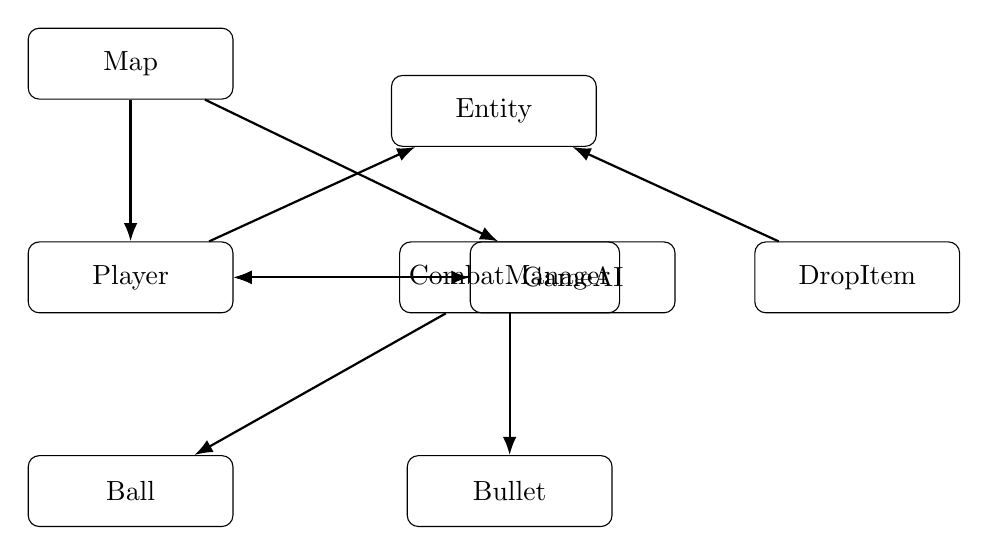
\begin{tikzpicture}[
  class/.style={rectangle, draw, rounded corners, align=center, minimum width=2.6cm, minimum height=0.9cm},
  rel/.style={-Latex, thick}
]
\node[class] (entity) {Entity};
\node[class, below left=1.2cm and 2.0cm of entity] (player) {Player};
\node[class, below right=1.2cm and 2.0cm of entity] (dropitem) {DropItem};
\node[class, right=3.0cm of player] (gameai) {GameAI};
\node[class, below=1.8cm of player] (ball) {Ball};
\node[class, right=2.2cm of ball] (bullet) {Bullet};
\node[class, above=1.8cm of bullet] (combat) {CombatManager};
\node[class, above=1.8cm of player] (map) {Map};

\draw[rel] (player) -- (entity);
\draw[rel] (dropitem) -- (entity);
\draw[rel] (gameai) -- (player);
\draw[rel] (combat) -- (player);
\draw[rel] (combat) -- (gameai);
\draw[rel] (combat) -- (ball);
\draw[rel] (combat) -- (bullet);
\draw[rel] (map) -- (player);
\draw[rel] (map) -- (gameai);
\end{tikzpicture}
\caption{核心类关系图。Entity 为基类，Ball、Bullet、DropItem 继承之；Player 与 Entity 分离，通过组合管理复杂状态；CombatManager、GameAI、Map 分别负责战斗结算、AI 决策和寻路，通过依赖关系与其他类协作。}
\label{fig:uml-minimal}
\end{figure}

\subsection{代码验证}

以下验证案例展示了多态和组合在实际运行中的表现：

\begin{longtable}{p{0.22\textwidth}p{0.34\textwidth}p{0.26\textwidth}p{0.12\textwidth}}
\toprule
\textbf{验证项} & \textbf{输入/触发} & \textbf{预期行为} & \textbf{结论} \\
\midrule
\endfirsthead
\toprule
\textbf{验证项} & \textbf{输入/触发} & \textbf{预期行为} & \textbf{结论} \\
\midrule
\endhead
多态渲染 & 玩家投掷实心球 + 开枪同时，场景中同时存在 Ball、Rifle Bullet、Sniper Bullet、DropItem & 所有实体通过同一段 \texttt{entity->draw()} 正确绘制各自贴图，无需类型判断 & 通过 \\
\hline
多态碰撞结算 & Ball 和 Bullet 分别击中玩家 & CombatManager 通过 \texttt{e->getWeaponType()} 和 \texttt{e->getDamage()} 获取不同的武器类型和伤害值，伤害公式各不同 & 通过 \\
\hline
多态生命周期管理 & 等待实体过期 & Ball 在飞行 3 秒后消失，Bullet 在飞行一定距离后消失，DropItem 在 300 帧后消失，全部通过同一个 \texttt{e->shouldBeRemoved()} 接口清理 & 通过 \\
\hline
组合模式词条叠加 & 玩家依次拾取"伤害+20\%"和"移速+15\%"词条 & ModifierState 中各字段独立累加，互不干扰，战斗计算统一遍历生效 & 通过 \\
\hline
继承与组合的边界 & 新增武器类型"狙击枪" & 只需在 WeaponType enum 中加一项 + switch 中加一个倍率分支，不需要新建类或修改 Entity 继承树 & 通过 \\
\bottomrule
\end{longtable}

\subsection{替代方案分析}

\begin{longtable}{p{0.22\textwidth}p{0.36\textwidth}p{0.36\textwidth}}
\toprule
\textbf{方案} & \textbf{优势} & \textbf{代价/为何未采用} \\
\midrule
\textbf{全部用独立类（无继承）} & 每个实体类型完全独立，无虚函数开销，编译依赖最小 & 需要在游戏循环的每个处理环节为每种实体写分支；新增实体需要在 10+ 个位置追加代码。对 4 种以上实体类型基本不可维护 \\
\hline
\textbf{Entity + Player 统一继承树} & Player 和 Entity 共享同一套更新/渲染接口 & Player 有动画状态机、输入系统、武器槽、词条等大量独有需求，强行套用 Entity 接口会让基类变得臃肿（要么塞进所有可能的方法让大部分子类留空，要么做大量 dynamic\_cast）。当前设计中 Player 和 Entity 分离是合理的 \\
\hline
\textbf{ECS 架构（Entity-Component-System）} & 完全的组件化设计，数据与行为彻底分离；System 遍历 Component 进行统一处理；极致灵活，运行时任意组合 & 架构复杂度和代码量远超当前需求（需要 Component 管理器、System 调度器、事件总线）；学习和调试成本高；在 6 种实体类型的规模下性价比低 \\
\hline
\textbf{ECS + 当前继承体系混合} & 更灵活 & 引入两种范式会增加概念负担和边界不一致，课程周期内不划算 \\
\bottomrule
\end{longtable}

\subsection{小结}

本项目的 OOP 应用遵循一条务实原则：\textbf{当多种对象共享生命周期和交互模式时，用继承消除重复；当对象的内部组成复杂但对外接口简单时，用组合管理复杂度；当类型间差异仅在于参数值时，用数据而非子类。}Entity 继承树处理了"多种飞行物/掉落物的统一更新渲染清理"，Player 的组合结构处理了"一个复杂角色的词条法术动画状态共存"，武器 enum 避免了不必要的继承开销。这三者结合，构成了项目中 OOP 技术应用的核心。

\newpage

% ============================================================
%  技术 2：事件驱动的模块间松耦合通信
% ============================================================
\section{技术二：事件驱动的模块间松耦合通信}

\subsection{游戏中引出的问题}

回顾游戏概览中列举的 10 个模块。如果把这些模块之间的信息流画出来，会得到一张相当复杂的图——

\begin{itemize}
  \item \textbf{PlayerController → Widget}：玩家按攻击键 → 创建投掷物实体（Ball 或 Bullet），添加到场景中
  \item \textbf{Widget → ModifierOverlay}：无尽模式每轮结束 → 弹出三选一词条面板；玩家做出选择 → 应用词条到玩家角色
  \item \textbf{Widget → EndlessResultWidget}：无尽模式死亡 → 显示结算面板；玩家点击按钮 → 返回菜单或重新开始
  \item \textbf{SetupWidget → MainWindow}：设置完成 → 携带 Session 配置启动游戏页面
  \item \textbf{Widget → MainWindow}：对局结束 → 通知主窗口切换页面
  \item \textbf{PlayerController → Widget}：定身被打破 → 通知 Widget 检查施法者是否有 CDR 词条以减少冷却
  \item \textbf{QTimer → Widget::gameLoop}：每 16ms 触发一次游戏帧，驱动整个游戏循环
\end{itemize}

如果不加设计地处理这些信息流，每个模块都会直接持有其他模块的指针并调用其方法。以"玩家开枪"为例：\texttt{PlayerController} 需要知道 \texttt{Widget} 的存在，调用 \texttt{widget->spawnBullet(x, y, vx, vy)}；如果后来又增加了音效模块和统计模块需要监听"开枪"事件，\texttt{PlayerController} 内部需要追加 \texttt{soundManager->playGunSound()} 和 \texttt{statsRecorder->recordShot()}。每个事件源都直接依赖所有事件消费者，依赖方向会变得不可预测。

更关键的是，这种直接调用方式意味着：\textbf{模块 A 必须知道模块 B 的完整接口。}如果将来把 Widget 换成另一个渲染器（比如从 QWidget 迁移到 QML），或者给 CombatManager 增加一个日志记录器，所有调用方都需要修改。这在只有 3-4 个模块时还能忍受——本项目 10+ 模块间的信息流如果全部走直接调用，修改任何一个消费者接口都会引发连锁修改。

\subsection{技术方案与设计思路}

解决上述问题的核心思路是\textbf{观察者模式}：事件源不直接调用消费者，而是"广播"一个信号出去，由消费者自己决定是否订阅。这种模式在不同平台有不同的实现——Qt 有 signal/slot，Boost 有 \texttt{signals2}，C\# 有 delegate/event，甚至 C 语言也能通过函数指针回调列表手动实现。无论哪种实现，本质都是\textbf{把"谁发出事件"和"谁来响应事件"解耦}。

\subsubsection{信号槽在本项目中的角色}

在 Qt 框架中，信号槽是语言级别的观察者模式实现：任何继承 \texttt{QObject} 的类都可以声明 \texttt{signals}（信号）并通过 \texttt{emit} 广播事件，\texttt{connect()} 负责建立信号到槽函数（或 lambda）的绑定。

本项目中，信号槽承担了三类通信角色：

\textbf{第一类：驱动帧循环的定时信号。}这是最高频的信号——每 16ms（约 60FPS）\texttt{QTimer::timeout} 触发 \texttt{Widget::gameLoop()}，整个游戏的"输入→逻辑→渲染"都在这个槽函数内顺序执行。信号在这里解决的是一个"周期性触发"的需求——如果用死循环加延时来做帧循环，Qt 的事件处理（包括接收键盘输入、重绘 UI）会被阻塞。

\begin{verbatim}
// widget.cpp 构造函数
timer = new QTimer(this);
connect(timer, &QTimer::timeout, this, &Widget::gameLoop);
// 启动后每 16ms 自动触发一次 gameLoop()
timer->start(16);
\end{verbatim}

\textbf{第二类：跨模块事件通知。}PlayerController 在检测到攻击指令时，不创建任何实体，只发出 \texttt{requestThrowBall} 信号并传参——调用方只需提供"谁在什么位置以什么速度发射了什么武器"。Widget 在连接这个信号后负责创建对应的实体对象。PlayerController 完全不知道 Entity 的存在。

\begin{verbatim}
// playercontroller.h —— 信号声明
signals:
    void requestThrowBall(float x, float y, float vx, float vy,
                          Player::WeaponType weapon, float damage,
                          float frozenBonus, int id);

// playercontroller.cpp —— 攻击时发出信号（节选）
if (player.lock()->weapon == Player::WeaponType::ball) {
    emit requestThrowBall(player.lock()->x, player.lock()->y,
                          player.lock()->vx, player.lock()->vy,
                          Player::WeaponType::ball,
                          getAttackDamage(), ...);
}

// widget.cpp —— 在游戏初始化时建立连接
connect(c1.get(), &PlayerController::requestThrowBall,
        this, &Widget::onPlayerRequest);
connect(c2.get(), &PlayerController::requestThrowBall,
        this, &Widget::onPlayerRequest);
\end{verbatim}

这个设计的关键价值在于：\textbf{PlayerController 和实体创建逻辑是完全隔离的。}PlayerController 只负责"报告攻击请求"，如果将来需要给攻击添加屏幕震动反馈或手柄振动，直接在 Widget 的 \texttt{onPlayerRequest} 槽函数中添加逻辑即可，PlayerController 一行代码都不需要改。

\textbf{第三类：页面间导航和状态同步。}游戏的页面流是 Setup → Game → Result，每次页面切换都涉及跨模块信息传递。例如 SetupWidget 完成设置后发出 \texttt{sessionReady(session)}，MainWindow 接收后隐藏设置页、创建游戏页并启动对局：

\begin{verbatim}
// mainwindow.cpp
connect(setupPage, &SetupWidget::sessionReady,
        this, &MainWindow::startGame);
\end{verbatim}

\subsubsection{动态连接与断开}

信号的另一个重要特性是可以\textbf{在运行时动态连接和断开}。本项目中广泛使用了这个能力——当游戏结束时断开定时器信号以停止帧循环，当结算面板关闭时断开其信号以防止悬空引用：

\begin{verbatim}
// 游戏结束，停止定时器
disconnect(timer, nullptr, this, nullptr);
// 结算面板关闭时断开其信号
disconnect(endlessResultWidget, nullptr, this, nullptr);
\end{verbatim}

以及用临时连接处理一次性事件——ModifierOverlay 弹出后，连接一次 \texttt{keyPressed} 信号，用户按任意键后立即断开：

\begin{verbatim}
connect(this, &Widget::keyPressed, overlay, [=]() {
    disconnect(this, &Widget::keyPressed, overlay, nullptr);
    // 处理按键 ...
});
\end{verbatim}

这种"接上-用过-断开"的模式避免了长期连接的累积，也防止了已经销毁的对象仍在接收信号导致崩溃。

\subsubsection{并非所有通信都用信号}

一个值得注意的设计选择是：项目并\textbf{没有}把所有模块间通信都交给信号槽。CombatManager 的战斗结算、SoundManager 的音效播放、Map 的碰撞查询，都通过直接函数调用完成。原因在于：

\begin{itemize}
  \item CombatManager 的结算函数在 gameLoop 中的执行时机是固定的（"先移动、后碰撞、最后结算"），消费者明确且唯一。信号槽的订阅/广播机制在这里是过度设计。
  \item SoundManager 的调用点分散在 CombatManager、PlayerController、Widget 三个模块中，但它是一个只读的全局服务——调用方自己决定什么时候播什么音效，不需要 SoundManager 反向通知调用方任何事。
\end{itemize}

这个区分体现了一个重要的工程判断：\textbf{信号槽适用于"一对多"和"未来可能有新消费者"的场景，而直接调用适用于"一对一"和"时机固定"的场景。}把信号槽用在该用的地方，而不是把它当银弹。

\subsection{代码验证}

\begin{longtable}{p{0.22\textwidth}p{0.34\textwidth}p{0.26\textwidth}p{0.12\textwidth}}
\toprule
\textbf{验证项} & \textbf{输入/触发} & \textbf{预期行为} & \textbf{结论} \\
\midrule
\endfirsthead
\toprule
\textbf{验证项} & \textbf{输入/触发} & \textbf{预期行为} & \textbf{结论} \\
\midrule
\endhead
发射信号-实体创建链路 & 玩家按键近战/投掷/射击，AI 触发攻击 & PlayerController 发出 requestThrowBall，Widget::onPlayerRequest 创建对应 Entity 并加入场景 & 通过 \\
\hline
定时信号驱动帧循环 & 游戏运行中 & QTimer::timeout → Widget::gameLoop 每 16ms 自动触发，帧率稳定在约 60FPS & 通过 \\
\hline
页面导航信号链 & 主菜单 → 设置 → 对局 → 结算 → 返回菜单 & SetupWidget::sessionReady → MainWindow::startGame；Widget::matchResultConfirmed → MainWindow::showMenu，信号驱动的页面切换全程无需模块间相互持有指针 & 通过 \\
\hline
动态断连防悬空 & 对局结束，定时器停止 & disconnect(timer, nullptr, ...) 后 gameLoop 不再被触发，无悬空引用或崩溃 & 通过 \\
\hline
词条选择信号 & 无尽模式每轮结束 & ModifierOverlay 弹出三选一，用户点击 optionChosen → Widget::onModifierChosen 应用词条到玩家，面板关闭 & 通过 \\
\bottomrule
\end{longtable}

\subsection{替代方案分析}

\begin{longtable}{p{0.22\textwidth}p{0.36\textwidth}p{0.36\textwidth}}
\toprule
\textbf{方案} & \textbf{优势} & \textbf{代价/为何未采用} \\
\midrule
\textbf{手动回调注册（函数指针或 std::function 列表）} & 无框架依赖；完全透明可见 & 需要手动管理回调列表（注册、注销、调用）；类型安全性靠程序员保证；链接错误不易排查。相当于自己实现一个粗糙版信号槽，维护成本高 \\
\hline
\textbf{事件总线 / 消息队列} & 全局消息通道，任何模块可发布和订阅；支持消息过滤和优先级；天然支持跨线程 & 引入额外的中间层和消息类型枚举；小型项目中增加复杂度多于收益；调试时消息路由不透明，难以追踪"谁响应了这个事件" \\
\hline
\textbf{全部使用直接函数调用} & 调用关系显式、IDE 可直接跳转、性能最优 & 每个模块都要持有所有可能消费者的指针或引用；依赖方向复杂；新加消费者需要改事件源代码。本项目的规模（10+ 模块）已经到了这个方案的维护边界 \\
\hline
\textbf{Qt 信号槽（当前方案）} & 观察者模式的语言级支持；类型安全（编译期检查信号与槽签名匹配）；支持动态连接/断开；Qt 框架内置，无需额外库 & 依赖 Qt 的 moc 预编译器和 Q\_OBJECT 宏；信号槽调用有轻微间接开销（对 60FPS 游戏可忽略）。本项目已使用 Qt 框架，边际成本为零 \\
\bottomrule
\end{longtable}

\subsection{小结}

信号槽在本项目中不是一个"用了 Qt 就顺便用一下"的功能，而是从模块间通信的复杂度出发推导出的必要方案。项目的实际使用方式也体现了选择性——高频固定的调用（如 CombatManager 结算）仍然走直接调用，只有"一对多""动态订阅""跨层级通知"的场景才用信号槽。这种"什么场景用什么通信方式"的判断，比"统一用信号槽"或"坚决不用信号槽"都更有价值。

\newpage

% ============================================================
%  技术 3：数据驱动的游戏玩法可扩展性
% ============================================================
\section{技术三：数据驱动的游戏玩法可扩展性}

\subsection{游戏中引出的问题}

格斗游戏需要"养成感"和"变化性"来支撑重复可玩性——尤其在无尽模式中，每一轮结束玩家从三个随机词条中选择一个，词条效果叠加，逐步变得更强；同时 AI 对手的强度也在递增。本项目的词条和法术系统加起来涉及：

\begin{itemize}
  \item \textbf{57 种词条类型}（15 种通用 + 42 种法术专属），按枚举 \texttt{ModifierType} 分类
  \item \textbf{6 种法术}（定身、隐身、安身、铜头铁臂、身外身、禁字法），各有不同的激活条件、持续时间和交互规则
  \item \textbf{30+ 个词条效果字段}集中在 \texttt{Player::ModifierState} 结构体中——移速倍率、各武器伤害倍率、减伤率、法术专属加成等
  \item \textbf{多层乘区叠加}：词条之间按独立乘区结算，同词条多级线性叠加
\end{itemize}

如果把这些全部硬编码进战斗代码，\texttt{getAttackDamage()} 会变成什么样子？每加一个词条就要加一个 if 分支，每加一个法术就要在伤害计算中插入一段特殊逻辑。57 种词条 × 5 种武器 × 6 种法术的排列组合将产生数百个需要维护的条件分支。

更关键的是可修改性问题：如果策划（或评阅老师）说"把定身增伤从 20\% 改成 25\%"，现在的做法是改 \texttt{modifierdata.h} 中的工厂方法里一个数值。如果全部硬编码，需要找到伤害计算函数中某一行埋在 500 行代码里的常量，还不敢保证改的是对的。

\subsection{技术方案与设计思路}

核心思路是\textbf{数据与逻辑分离}：用结构体描述"词条是什么"，玩家状态字段存储"词条产生了什么效果"，战斗逻辑代码\textbf{遍历}状态字段来结算——战斗逻辑本身不包含任何词条的细节。

\subsubsection{三个层次的数据驱动设计}

\textbf{第一层：词条数据的定义（ModifierData）。}文件 \texttt{modifierdata.h} 将每类词条封装为一个 \texttt{ModifierData} 结构：

\begin{verbatim}
struct ModifierData {
    ModifierType type;
    QString      displayName;   // 卡片标题，如"急转轮回"
    QString      description;   // 卡片描述，如"法术冷却 -5秒"
    int          level = 1;
};

enum class ModifierType {
    SPELL_COOLDOWN_REDUCE, MAX_HP_UP, ENEMY_MAX_HP_DOWN,
    MOVE_SPEED_UP, ENEMY_MOVE_SPEED_DOWN,
    PUNCH_DAMAGE_UP, KNIFE_DAMAGE_UP, BALL_DAMAGE_UP, GUN_DAMAGE_UP,
    DAMAGE_BONUS_UP, DAMAGE_REDUCTION_UP,
    DOUBLE_EDGE, EXTRA_WEAPON_SLOT,
    FREEZE_DURATION_UP, FREEZE_DAMAGE_UP, FREEZE_BREAK_CDR,
    STEALTH_DURATION_UP, STEALTH_SPEED_UP, STEALTH_REGEN, STEALTH_FIRST_HIT,
    // ... 其余 30+ 种
};
\end{verbatim}

工厂方法 \texttt{poolForPlayer(spellName)} 根据玩家的法术类型返回合法的词条池——通用词条 + 法术专属词条。例如定身法玩家会看到"急转轮回""长缚""破而后立"等，不会看到隐身专属的"破影一击"。

\begin{verbatim}
// 工厂方法示例：按法术返回专属词条
inline QVector<ModifierData> ModifierData::forSpell(const QString& spellName) {
    if (spellName == "freeze") {
        return {
            { FREEZE_DURATION_UP,  "长缚",     "定身持续时间 +1.5秒" },
            { FREEZE_DAMAGE_UP,    "缚中伤",   "定身期间伤害 +20%" },
            { FREEZE_BREAK_CDR,    "破而后立", "定身破碎后冷却 -5秒（唯一）" },
        };
    }
    if (spellName == "stealth") {
        return { /* 隐身专属词条 */ };
    }
    // ...
}
\end{verbatim}

\textbf{第二层：玩家状态字段（ModifierState）。}Player 内部维护一个 \texttt{ModifierState modifiers} 结构体，包含所有词条生效后的数值累加结果：

\begin{verbatim}
struct ModifierState {
    int   spellCooldownReduce   = 0;
    float maxHpMultiplier       = 1.0f;
    float moveSpeedMultiplier   = 1.0f;
    float punchDmgMultiplier    = 1.0f;
    float knifeDmgMultiplier    = 1.0f;
    float ballDmgMultiplier     = 1.0f;
    float gunDmgMultiplier      = 1.0f;
    float damageBonusMultiplier = 1.0f;
    float damageReduction       = 0.0f;
    bool  doubleEdge            = false;
    float freezeDurationBonus   = 0.f;
    float freezeDmgMultiplier   = 1.0f;
    bool  freezeBreakCDR        = false;
    // ... 30+ fields
};
\end{verbatim}

\textbf{第三层：词条应用到状态字段（applyModifier）。}当玩家拾取词条时，\texttt{Player::applyModifier(const ModifierData\& mod)} 根据 \texttt{mod.type} 将数值累加到对应的状态字段：

\begin{verbatim}
void Player::applyModifier(const ModifierData& mod) {
    switch (mod.type) {
    case ModifierType::SPELL_COOLDOWN_REDUCE:
        modifiers.spellCooldownReduce += 5;
        spellState.cooldownMax    = qMax(5.f, spellState.cooldownMax - 5.f);
        spellState.cooldownRemain = qMax(0.f, spellState.cooldownRemain - 5.f);
        break;
    case ModifierType::DAMAGE_BONUS_UP:
        modifiers.damageBonusMultiplier += 0.25f;  break;
    case ModifierType::DAMAGE_REDUCTION_UP:
        modifiers.damageReduction = qMin(0.6f, modifiers.damageReduction + 0.2f);
        break;
    case ModifierType::DOUBLE_EDGE:
        modifiers.doubleEdge = true;  break;
    // ... 50+ cases
    }
}
\end{verbatim}

这个 switch 是整个系统中\textbf{唯一}需要了解词条类型到状态字段对应关系的地方。\textbf{战斗代码完全不碰 ModifierType 枚举。}

\textbf{战斗代码消费的是状态字段，不是词条类型。}\texttt{getAttackDamage()} 展示的就是这一层：

\begin{verbatim}
float Player::getAttackDamage() {
    float base = 0.f;
    switch (weapon) {
    case WeaponType::punch:  base = 5.f  * modifiers.punchDmgMultiplier; break;
    case WeaponType::knife:  base = 15.f * modifiers.knifeDmgMultiplier; break;
    case WeaponType::ball:   base = 1.f  * modifiers.ballDmgMultiplier;  break;
    // ...
    }
    base *= modifiers.damageBonusMultiplier;
    if (modifiers.doubleEdge) base *= 1.5f;
    // 隐身破影一击有额外的随时间增长伤害倍率
    if (spellState.stealthActive && modifiers.stealthFirstHit && ...) {
        float ratio = qMin(elapsed / totalDuration, 1.0f);
        base *= (1.0f + ratio);
    }
    return base;
}
\end{verbatim}

注意：\texttt{getAttackDamage()} 不知道"伤害+20\%"是哪来的——它只看到 \texttt{damageBonusMultiplier} 字段当前值是 1.25（吃了一个词条），它无法也不需区分这是"DAMAGE\_BONUS\_UP"还是"FORBIDDEN\_WORD"贡献的。这就是数据驱动的本质：\textbf{战斗逻辑对数据来源保持无知}。

\subsubsection{SpellState：法术状态的纯数据结构}

法术相关的运行时状态也设计为纯数据结构（\texttt{spellstate.h}），不含任何业务逻辑：

\begin{verbatim}
struct SpellState {
    float cooldownRemain = 0.f;   // 剩余冷却时间
    float cooldownMax    = 0.f;
    bool  isFrozen       = false; // 是否被定身
    float frozenRemain   = 0.f;
    bool  stealthActive  = false; // 隐身是否激活
    float stealthRemain  = 0.f;
    bool  ironBodyActive = false; // 铜头铁臂是否激活
    // ... 其他法术状态

    void tick(float dt) {
        // 所有定时器统一递减，到零自动关闭状态
        if (cooldownRemain > 0.f) cooldownRemain -= dt;
        if (frozenRemain   > 0.f) { frozenRemain -= dt;
            if (frozenRemain <= 0.f) isFrozen = false; }
        // ...
    }
};
\end{verbatim}

\begin{quote}
\small 注释：tick() 中直接写了递减逻辑，未抽象为虚函数。原因是有 6 种法术计时器共享完全相同的行为（递减 → 触零 → 关闭标志），抽象为虚函数只会增加代码跳转次数而不减少任何重复。这是数据驱动设计中的一个务实判断：\textbf{当数据的"结构"一样时，不值得为结构相同的类型引入多态}。
\end{quote}

\begin{figure}[H]
\centering
\begin{tikzpicture}[
  node distance=0.95cm,
  box/.style={rectangle, draw, rounded corners, align=center, minimum width=3.5cm, minimum height=0.75cm},
  arr/.style={-Latex, thick}
]
\node[box] (hit) {碰撞有效};
\node[box, below=of hit] (attacker) {获取攻击者属性（ModifierState、武器类型）};
\node[box, below=of attacker] (defender) {获取防守者属性（护甲、ModifierState、法术状态）};
\node[box, below=of defender] (base) {基础伤害 = 武器倍率 × 词条加成};
\node[box, below=of base] (modifier) {通用伤害加成 / 两败俱伤 / 定身受击增伤};
\node[box, below=of modifier] (armor) {护甲减伤后置衰减};
\node[box, below=of armor] (stagger) {计算硬直时间（按伤害等级查表）};
\node[box, below=of stagger] (reflection) {铜头铁臂反弹判定};
\node[box, below=of reflection] (apply) {应用伤害与状态};

\draw[arr] (hit) -- (attacker);
\draw[arr] (attacker) -- (defender);
\draw[arr] (defender) -- (base);
\draw[arr] (base) -- (modifier);
\draw[arr] (modifier) -- (armor);
\draw[arr] (armor) -- (stagger);
\draw[arr] (stagger) -- (reflection);
\draw[arr] (reflection) -- (apply);
\end{tikzpicture}
\caption{伤害计算流水线。注意：每一步消费的都是 ModifierState 中的数值字段，而非 ModifierType 枚举——这正是技术三"数据驱动"的关键：战斗代码对词条来源保持无知。}
\label{fig:damage-calc}
\end{figure}

\subsection{代码验证}

\begin{longtable}{p{0.22\textwidth}p{0.34\textwidth}p{0.26\textwidth}p{0.12\textwidth}}
\toprule
\textbf{验证项} & \textbf{输入/触发} & \textbf{预期行为} & \textbf{结论} \\
\midrule
\endfirsthead
\toprule
\textbf{验证项} & \textbf{输入/触发} & \textbf{预期行为} & \textbf{结论} \\
\midrule
\endhead
词条池生成 & 定身法玩家进入无尽模式 & \texttt{poolForPlayer("freeze")} 返回 13 通用 + 3 法术专属，不包含隐身/安身等无关词条 & 通过 \\
\hline
词条叠加 & 连续拾取两次"伤害加成+25\%" & ModifierState.damageBonusMultiplier = 1.5，getAttackDamage 返回伤害 = 基础 × 1.5 & 通过 \\
\hline
唯一词条 & 尝试多次获取"两败俱伤" & isUniqueModifier 返回 true，UI 层阻止重复选择 & 通过 \\
\hline
新词条零影响战斗代码 & 新增"护甲穿透"词条 & 只需在 enum 加一项 + applyModifier 加一个 case + ModifierState 加一个字段；getAttackDamage 和 CombatManager 完全不改 & 通过 \\
\hline
法术定时器统一 tick & 冻结、隐身、铜头同时激活 & SpellState::tick(dt) 统一递减所有计时器，到期自动关闭对应标志 & 通过 \\
\bottomrule
\end{longtable}

\subsection{替代方案分析}

\begin{longtable}{p{0.22\textwidth}p{0.36\textwidth}p{0.36\textwidth}}
\toprule
\textbf{方案} & \textbf{优势} & \textbf{代价/为何未采用} \\
\midrule
\textbf{全部硬编码（if-else 分支）} & 直接明了，IDE 可跳转 & 57 种词条 × 多处消费点 = 代码爆炸；新增词条需要改动 combat + UI + 记录等所有涉及模块 \\
\hline
\textbf{脚本化（Lua/Python 嵌入）} & 策划可独立修改数值和行为逻辑而不需 C++ 编译 & 需要集成脚本解释器和 C++ ↔ 脚本绑定层；调试变复杂（C++ 调用栈 + 脚本调用栈混合）；课程周期内投入产出比低 \\
\hline
\textbf{JSON/配置表驱动} & 词条数据完全外部化（文本文件），非程序员可编辑 & 需要解析器和错误处理；加载失败时的降级策略需额外设计；运行时类型安全不如编译期 enum \\
\hline
\textbf{当前方案（enum + struct + switch）} & 编译期类型检查；新增词条只需改一个 switch；战斗代码对来源无知；无外部依赖 & 词条数量达到 100+ 时，applyModifier 的 switch 会变长；但 57 种量级完全可控 \\
\bottomrule
\end{longtable}

\subsection{小结}

本项目的词条与法术系统通过三层数据驱动架构（定义层 ModifierData → 状态层 ModifierState → 消费层 getAttackDamage）实现了可扩展性。关键设计决策是\textbf{不让战斗代码知道词条类型}——战斗逻辑只读状态字段，不关心字段值从哪来。这个决策使"新增一种词条"的成本从"修改多个模块"降为"修改一个 enum 和一个 switch case"。

\newpage

% ============================================================
%  技术 4：有限状态机驱动的 NPC 决策
% ============================================================
\section{技术四：有限状态机驱动的 NPC 决策}

\subsection{游戏中引出的问题}

单局对战模式中，AI 需要扮演一个"像人"的对手。一个简单的跟随+攻击脚本——"看到玩家就冲过去打"——在静态环境中或许勉强可用，但这个游戏中有如下变量：

\begin{itemize}
  \item 玩家可能隐身后绕到侧面偷袭，AI 需要处理"看不见目标"的情况
  \item 地面可能刷新更好的武器或词条，AI 需要判断"是继续打还是先去捡"
  \item AI 血量低时需要考虑撤退、找补给或换策略
  \item 地图上移动路径可能被阻隔（平台间需要寻路跳转），也可能卡在平台边缘反复抖动
  \item 释放法术后应该有一段"乘胜追击"的窗口，而不是放完技能立刻摆烂
  \item AI 不能太强（玩家感受极差），也不能太弱（无聊），需要对不同水平的玩家有区分度
\end{itemize}

这些问题无法用一串 if-else 解决——决策条件会指数级交叉（"血量低 AND 对手隐身 AND 地上有狙击枪 AND 我正在卡住 → 怎么办？"）。需要一个结构化的决策框架。

\subsection{技术方案与设计思路}

本项目的 AI 采用了\textbf{分层的有限状态机 + 特殊分支优先}的架构。核心思想是：常规战术行为交给状态机轮流执行，但紧急或特殊事件（隐身、卡住、施法后追击）直接跳出状态机走独立处理路径。

\subsubsection{三层决策架构}

\begin{verbatim}
// gameai.cpp — updateIntent() 的主流程（简化版）
void GameAI::updateIntent(MoveIntent& moveIntent, AttackIntent& attackIntent) {
    moveIntent = MoveIntent::NONE; attackIntent = false;

    // ── 第一层：特殊策略（优先级最高，跳过状态机） ──
    if (隐身 + 破影一击) { executeStealthFirstHitStrategy(...); return; }
    if (!目标可见)        { handleStealthTarget(...);            return; }
    if (卡住了)           { handleStuckSituation(moveIntent);    return; }
    if (正在执行动作计划) { 弹出下一帧动作，return;            }

    // ── 第二层：状态机执行 ──
    switch (m_currentState) {
    case AIState::FOLLOW:       executeFollow(moveIntent, ...); break;
    case AIState::ATTACK:       executeAttack(moveIntent, ...); break;
    case AIState::SEEK_WEAPON:  executeSeekWeapon(...);       break;
    //  ... 共 8 个状态
    }

    // ── 第三层：状态转换 ──
    AIState nextState = determineNextState();
    if (nextState != m_currentState) m_currentState = nextState;
}
\end{verbatim}

这个结构清晰地划分了三个优先层级：

\begin{enumerate}
  \item \textbf{特殊策略层}："活下来"的需求优先于"打得聪明"。隐身、卡住、执行预定计划等情况直接劫持流程，不经过状态机。这避免了状态机在异常情况下做出不合理的切换（比如隐身时 AI 跑去"找武器"而不是搜索最后已知位置）。
  \item \textbf{状态机层}：在正常情况下，由当前状态对应的执行函数生成 MoveIntent 和 AttackIntent。每个状态只关心"当前状态下我该做什么"——FOLLOW 负责寻路接近目标，ATTACK 负责判定距离并发动攻击，SEEK\_WEAPON 负责朝最优武器掉落位置移动。
  \item \textbf{状态转换层}：\texttt{determineNextState()} 在每帧末尾评估全局局势，决定是否切换状态。转换评估与执行是分离的——当前状态的执行函数不关心"下一帧会不会换状态"。
\end{enumerate}

\subsubsection{状态转换的决策逻辑}

\texttt{determineNextState()} 是本系统的核心（约 85 行），综合评估多项条件来决定状态切换：

\begin{itemize}
  \item \textbf{是否无法伤害对手}（canDamageTarget）：拳击打链甲无效、弹药耗尽等情况 → 优先找武器
  \item \textbf{地面上是否有更好的物资}（hasWeaponDrop / hasArmorDrop / hasSupplyDrop）→ 降低攻击倾向，提升搜索倾向
  \item \textbf{有无尽模式}：无尽模式中移除了"低血量撤退"逻辑（因为 AI 有 endlessImmortal 可复活），改为纯概率驱动
  \item \textbf{血量比例}（healthRatio $\leq 32\%$）：触发人格分化——"背水一战"人格继续打，"游走机动"人格撤退找药
  \item \textbf{长期目标锁}（GOAL\_LOCK\_DURATION）：每约 10 秒通过 \texttt{refreshStrategicGoal()} 重新抛骰子决定"进攻为主"还是"搜刮为主"，锁定期内不频繁切换，避免帧间抖动
\end{itemize}

\textbf{人格系统}为决策注入了可控的随机性。AI 出生时随机分配两种人格之一：
\begin{itemize}
  \item \textbf{BACK\_TO\_WALL（背水一战）}：低血量时仍倾向进攻，搜刮倾向低（25\%-35\%）
  \item \textbf{KITE\_SCAVENGER（游走机动）}：低血量时大幅提升搜刮概率（60\%-80\%），优先找补给和装备
\end{itemize}

人格设计的目的不是让 AI "聪明"，而是让\textbf{每次对局的 AI 行为不可预测}。相同配置下，不同人格的 AI 会给玩家完全不同的感觉。

\subsubsection{特殊分支的实际价值}

\textbf{卡住检测与脱困}是特殊分支中最直接体现工程价值的。AI 在复杂平台地形中可能卡在边缘反复左右晃动。检测方式：连续多帧位移小于阈值 → 判为卡住 → 清空动作计划 → 执行脱困跳跃。这个逻辑完全跳过状态机，无论当前是什么状态，都能第一时间响应，极大提升了 AI 的流畅度和玩家的体验。

\textbf{施法后强制攻击模式}解决了一个微妙的时序问题：AI 释放法术后，如果下一帧 \texttt{determineNextState()} 评估为"距离太远要跟随"，法术的战略价值就白费了。因此在 \texttt{executeFollow()} 内部插入了一段施法后的强制逻辑——法术释放后的 60 帧内强制保持攻击态势，靠近对手并连续攻击。

\textbf{隐身目标处理}则展示了状态机覆盖不到的边缘情况。玩家隐身时，AI 不再用状态机跟踪目标，而是前往玩家隐身前的最后已知位置巡逻。如果AI带"破影一击"词条，AI 还有专门的前期积攒物资、最后时机出手的策略。

\begin{figure}[H]
\centering
\begin{tikzpicture}[
  node distance=1.1cm,
  box/.style={rectangle, draw, rounded corners, align=center, minimum width=3.2cm, minimum height=0.8cm},
  arr/.style={-Latex, thick}
]
\node[box] (special) {特殊分支优先：隐身 / 卡住 / 施法后追击};
\node[box, below=of special] (sense) {感知环境（目标位置、可见性、掉落物）};
\node[box, below=of sense] (state) {determineNextState：评估血量/物资/人格};
\node[box, below left=0.9cm and 1.6cm of state] (attack) {ATTACK：近战/远程};
\node[box, below=of state] (follow) {FOLLOW：寻路追击};
\node[box, below right=0.9cm and 1.6cm of state] (seek) {SEEK\_WEAPON/ARMOR/SUPPLY};
\node[box, below=2.0cm of state] (recover) {卡住脱困 / 施法后强制攻击};

\draw[arr] (special) -- (sense);
\draw[arr] (sense) -- (state);
\draw[arr] (state) -- (attack);
\draw[arr] (state) -- (follow);
\draw[arr] (state) -- (seek);
\draw[arr] (attack) -- (sense);
\draw[arr] (follow) -- (sense);
\draw[arr] (seek) -- (sense);
\draw[arr] (state) -- (recover);
\draw[arr] (recover) -- (sense);
\end{tikzpicture}
\caption{AI 决策流程。顶层特殊分支（隐身/卡住/施法后追击）直接跳过状态机；正常流程走感知 → 状态转换评估 → 状态执行；卡住和施法后强制模式为独立路径，不受状态机当前状态影响。}
\label{fig:ai-flow}
\end{figure}

\subsection{代码验证}

\begin{longtable}{p{0.22\textwidth}p{0.34\textwidth}p{0.26\textwidth}p{0.12\textwidth}}
\toprule
\textbf{验证项} & \textbf{输入/触发} & \textbf{预期行为} & \textbf{结论} \\
\midrule
\endfirsthead
\bottomrule
\endhead
FOLLOW 状态寻路 & 玩家在地图另一端 & AI 通过 Map BFS 算出平台序列，生成朝向玩家的移动意图，遇到平台边缘自动跳跃 & 通过 \\
\hline
状态切换 & AI 血量降至 30\% + 人格为 KITE\_SCAVENGER & determineNextState 返回 RETREAT 或 SEEK\_SUPPLY，AI 从攻击转为撤退/搜刮 & 通过 \\
\hline
卡住脱困 & AI 卡在平台边缘连续 100 帧位移 < 5 像素 & isStuck() 返回 true → handleStuckSituation 清空动作计划并执行跳跃脱困 & 通过 \\
\hline
施法后追击 & AI 释放定身法命中玩家 & 进入 60 帧强制攻击窗口，AI 朝被定身的玩家移动并持续输出，不会切回 FOLLOW & 通过 \\
\hline
隐身搜索 & 玩家激活隐身 & AI 保存最后已知位置，前往该位置附近巡逻，不会呆立原地 & 通过 \\
\hline
人格分化 & 同一配置对局两局 & 两局 AI 人格可能不同（出生时随机），导致低血量时行为截然不同 & 通过 \\
\bottomrule
\end{longtable}

\subsection{替代方案分析}

\begin{longtable}{p{0.22\textwidth}p{0.36\textwidth}p{0.36\textwidth}}
\toprule
\textbf{方案} & \textbf{优势} & \textbf{代价/为何未采用} \\
\midrule
\textbf{纯 if-else 决策树} & 无框架开销，直接 & 条件组合爆炸（血量 × 可见性 × 物资 × 地形），维护不可持续 \\
\hline
\textbf{行为树（Behavior Tree）} & 模块化决策节点，易于可视化和组合；Unreal Engine 等引擎内置支持 & 实现一个可用的行为树框架本身就需要大量代码（节点基类、组合节点、装饰器、黑板）；对 C++ 课程项目来说，实现行为树的成本已超过调试 AI 行为的成本 \\
\hline
\textbf{GOAP/规划器} & 最优动作序列搜索，理论上能产生更智能的行为 & 实现极其复杂，且规划结果不可预测，调试困难。对于 8 状态的小型状态机，规划器过度设计 \\
\hline
\textbf{当前方案（分层 FSM）} & 实现成本低；状态边界清晰，出问题能快速定位是"特殊分支""状态机"还是"状态转换"的 bug；预留了 8 个状态的扩展空间 & 状态增多时转换矩阵变复杂；相较行为树，表达并行行为（一边移动一边射击）不够自然——本项目中通过"施法后强制模式"这类特殊分支补偿了这个弱点 \\
\bottomrule
\end{longtable}

\subsection{小结}

有限状态机在本项目中不是"最先进的 AI 技术"，但它足够胜任 8 个状态 + 4 个特殊分支的决策空间，且在课程周期内能以最低的代码量提供可区分的 AI 行为。关键设计是\textbf{特殊分支跳过状态机}和\textbf{目标锁定防抖动}——前者处理紧急情况，后者防止决策在相邻帧之间反复切换。加上人格系统注入的随机性，FSM 驱动的 AI 在有限的复杂度下交出了"不可预测且可维护"的答卷。

\newpage

% ============================================================
%  技术 5：实时游戏主循环的时序设计
% ============================================================
\section{技术五：实时游戏主循环的时序设计}

\subsection{游戏中引出的问题}

格斗游戏的实时性要求极高。一帧 16ms 内要完成：读取键盘输入 → AI 决策 → 移动角色 → 碰撞检测 → 伤害结算 → 生成/清理实体 → 播放音效 → 重绘屏幕。这些子系统之间存在严格的时序依赖：

\begin{itemize}
  \item 碰撞检测\textbf{必须}在移动之后执行——否则检测的是上一帧的位置，"子弹穿透角色"会频繁出现
  \item 死亡检查\textbf{必须}在伤害结算之后——结算前检查会导致"最后一击"被跳过
  \item 实体清理\textbf{必须}在所有计算完成后——提前清理会让还在空中的子弹在被命中判定前消失
  \item 帧时间 dt 必须基于真实耗时——如果机器卡顿了一帧（比如 0.1s 而不是 0.016s），角色的移动距离和冷却计时需要同步放大，否则会出现"时间变慢"的观感
\end{itemize}

简单地把所有模块扔进一个 while 循环而不管理执行顺序，会导致各种难以复现的 bug：子弹偶尔穿透、死亡触发时机不一致、卡顿后行为异常。这些 bug 的共同特征是\textbf{不稳定}——同样的攻击有时命中有时穿透，给调 bug 带来极大痛苦。

\subsection{技术方案与设计思路}

\subsubsection{固定的帧更新流水线}

本项目的 gameLoop 函数约 40 行，但其中包含了一个严格顺序的流水线。下面展示完整流程（注释中标记了每个步骤的目的和时序依赖）：

\begin{verbatim}
void Widget::gameLoop() {
    // ── 1. 计算真实帧时间（处理卡顿补偿） ──
    float dt = lastTime.restart() / 1000.0f;
    m_gameTime += dt;

    // ── 2. 计时器与生成逻辑 ──
    //     无尽模式 AI 定时获取词条、随机生成掉落物
    if (currentSession.mode == GameSession::Mode::ENDLESS) {
        m_endlessAiModifierTimer += dt;
        if (m_endlessAiModifierTimer >= ENDLESS_AI_MODIFIER_INTERVAL)
            applyRandomModifierToAI();
    }
    spawnDrop();       // 每帧尝试生成掉落物
    updateDrops(dt);   // 更新已有掉落物计时

    // ── 3. 死亡检查（伤害结算之前不能做） ──
    if (players[0]->isDead()) { gameEnd(1); return; }
    if (players[1]->isDead()) { gameEnd(0); return; }

    players[0]->setDt(dt); players[1]->setDt(dt);

    // ── 4. AI 决策（生成意图，不执行移动） ──
    ai->updateIntent(moveIntent, attackIntent);
    intent[1].moveIntent    = moveIntent;
    intent[1].attackIntent  = attackIntent;

    // ── 5. 执行移动（玩家 + AI） ──
    controllers[0]->handleIntent(intent[0].moveIntent, ...);
    controllers[1]->handleIntent(intent[1].moveIntent, ...);

    // ── 6. 碰撞检测与战斗结算 ──
    //     位置已更新，此时碰撞检测的是"最新位置"
    cm.checkPlayerVsPlayerCollision(controllers[0], controllers[1]);
    updateBalls(dt);    // 飞行物移动 + 碰撞检测

    // ── 7. 状态更新 ──
    tickSpells(dt);     // 法术冷却递减

    // ── 8. 清理过期对象（所有结算完成后） ──
    entities.erase(std::remove_if(entities.begin(), entities.end(),
                   [](auto& e) { return e->shouldBeRemoved(); }),
                   entities.end());

    // ── 9. 触发重绘（paintEvent） ──
    update();
}
\end{verbatim}

这个时序设计的核心原则是：\textbf{信息在帧内单向流动，不做跨步骤回写。}步骤 1-3 收集信息，步骤 4-5 更新位置，步骤 6 基于最新位置结算，步骤 7-9 做收尾和展示。如果步骤 6 修改了某个实体的位置（比如反弹），被反弹的实体位置变化会在下一帧的步骤 5 中生效——不会出现"同一帧内两个步骤并发修改导致不一致"的问题。

\subsubsection{帧时间补偿（dt 传递）}

卡顿是不可避免的——垃圾回收、操作系统调度、磁盘 IO 都可能阻塞一帧。本项目中 dt 的传递路径是：

\begin{center}
\texttt{lastTime.restart() → float dt → players[i]->setDt(dt) → Entity::setDt(dt) → 物理公式}
\end{center}

在 \texttt{applyGravity()} 中，位置更新用的是 $v_y = v_y + g \cdot dt$ 而非 $v_y = v_y + g \cdot 0.016$。如果 dt = 0.1s（卡顿了 6 帧），角色会跳跃 $0.1 / 0.016 \approx 6$ 倍的距离，补偿了丢失的时间。这个方法叫\textbf{可变时间步长}（variable timestep），优点是实现简单且卡顿后位置一致性不丢失，缺点是物理模拟不是严格确定性的（两次运行因 dt 微小差异可能产生略有不同的轨迹）。对本项目这种不要求帧精确复现的格斗游戏，这个代价是可接受的。

\subsubsection{对象生命周期管理}

球和子弹是瞬态对象（击中后立即删除），但删除时机不当会导致悬挂指针或 double-free。本项目使用 \texttt{std::shared\_ptr<Entity>} 统一管理实体对象，配合 \texttt{std::weak\_ptr} 在掉落物和球容器中存储弱引用：

\begin{verbatim}
std::vector<std::shared_ptr<Entity>> entities;  // 所有实体（拥有所有权）
std::vector<std::weak_ptr<Ball>> balls;          // 球引用（不拥有所有权）
std::vector<std::weak_ptr<DropItem>> drops;     // 掉落物引用（不拥有所有权）
\end{verbatim}

每帧末尾通过 \texttt{remove\_if + shouldBeRemoved()} 清理 entities 中的过期对象，同时用 \texttt{weak\_ptr::expired()} 清理 balls 和 drops 中已失效的引用。这个机制的优点是：balls 容器中的引用在 entity 被销毁后自动变空，不会出现"拿到指针但对象已经被删除"的情况。

\begin{figure}[H]
\centering
\begin{tikzpicture}[
  node distance=1.0cm,
  box/.style={rectangle, draw, rounded corners, align=center, minimum width=3.8cm, minimum height=0.8cm},
  arr/.style={-Latex, thick}
]
\node[box] (event) {输入或碰撞事件};
\node[box, below=of event] (check) {命中判定与目标验证};
\node[box, below=of check] (damage) {伤害计算 + 词条遍历 + 硬直查表};
\node[box, below=of damage] (update) {更新血量、状态、法术冷却};
\node[box, below=of update] (cleanup) {清理过期实体（remove\_if + shouldBeRemoved）};
\node[box, below=of cleanup] (feedback) {重绘（update → paintEvent）+ 音效播放};

\draw[arr] (event) -- (check);
\draw[arr] (check) -- (damage);
\draw[arr] (damage) -- (update);
\draw[arr] (update) -- (cleanup);
\draw[arr] (cleanup) -- (feedback);
\end{tikzpicture}
\caption{单帧执行流水线。箭头表示信息流动方向——前一步的输出是后一步的输入。所有步骤在当前帧内顺序执行，不跨步骤回写，保证每个步骤操作的数据在帧内是一致的。}
\label{fig:combat-flow}
\end{figure}

\subsection{代码验证}

\begin{longtable}{p{0.22\textwidth}p{0.34\textwidth}p{0.26\textwidth}p{0.12\textwidth}}
\toprule
\textbf{验证项} & \textbf{输入/触发} & \textbf{预期行为} & \textbf{结论} \\
\midrule
\endfirsthead
\bottomrule
\endhead
碰撞时序 & 玩家和 AI 同时朝对方冲刺并出拳 & 碰撞在双方移动后结算，命中判定基于最新位置，不会出现"打空气命中"或"穿透" & 通过 \\
\hline
卡顿补偿 & 模拟帧卡顿（强制 sleep 50ms） & dt 变大，角色跳跃高度和移动距离同步放大，不出现"画面停顿但逻辑加速"的现象 & 通过 \\
\hline
对象安全清理 & 投掷球飞行 3 秒后自动消失 & entities 末尾 remove\_if 清理，balls 中的 weak\_ptr::expired 返回 true，同步清理弱引用 & 通过 \\
\hline
死亡检查时序 & 双方同时对最后一击 & 伤害结算完成后才检查 isDead，不存在"击杀了但伤害没扣"的情况 & 通过 \\
\bottomrule
\end{longtable}

\subsection{替代方案分析}

\begin{longtable}{p{0.22\textwidth}p{0.36\textwidth}p{0.36\textwidth}}
\toprule
\textbf{方案} & \textbf{优势} & \textbf{代价/为何未采用} \\
\midrule
\textbf{固定时间步长（Fixed Timestep）} & 物理模拟严格确定性，回放和录像可精确复现 & 需要累积器（accumulator）机制，额外的代码复杂度；慢帧会导致"螺旋式死亡"（多帧积压同时结算）。本项目的精度需求不要求帧精确复现 \\
\hline
\textbf{多线程游戏循环} & 可利用多核并行处理物理/AI/渲染 & 线程同步会极大增加复杂度（锁、原子操作、数据竞争）；对于 60FPS 的 2D 游戏，单线程已足够支撑所有计算 \\
\hline
\textbf{当前方案（单线程可变 dt 流水线）} & 实现极简，时序完全可控，调试路径清晰 & 物理非确定性的代价；如果未来加入联网对战或录像回放，需要改为固定时间步长 \\
\bottomrule
\end{longtable}

\subsection{小结}

游戏主循环的时序设计本质上是一个\textbf{信息流编排问题}：在每 16ms 的时间窗口内，如何安排子系统执行顺序使得每步计算都基于"最新且一致"的信息。本项目的方案选择了最简单可维护的路径——单线程、固定顺序、可变时间步长——在 60FPS 要求下稳定运行，且调试时卡在某一步可以精确知道哪些数据已经更新、哪些还没变。

\newpage

% ============================================================
%  技术 6：跨平台构建系统的抽象与配置
% ============================================================
\section{技术六：跨平台构建系统的抽象与配置}

\subsection{游戏中引出的问题}

这个游戏的源代码组织面临一个"纯代码之外"的工程问题。项目包含：

\begin{itemize}
  \item 40+ 个源文件（.h / .cpp），分布在 10 个模块中
  \item 依赖 Qt 6 的三个独立模块：Widgets、Multimedia、Core
  \item 一个 Qt 资源文件（.qrc）管理图片和音效资源
  \item 需要在 Windows（MinGW）和 macOS 上都能编译
  \item 使用 C++17 标准（结构化绑定、\texttt{std::optional}、\texttt{if constexpr} 等特性）
  \item MSVC 编译器需要处理 UTF-8 中文注释的编码
\end{itemize}

如果手动管理编译，典型的一条 g++ 编译命令会是：

\begin{verbatim}
g++ -std=c++17 -I/path/to/Qt6/include -I/path/to/Qt6/include/QtWidgets
    -I/path/to/Qt6/include/QtCore -I/path/to/Qt6/include/QtMultimedia
    -L/path/to/Qt6/lib -lQt6Widgets -lQt6Core -lQt6Multimedia
    main.cpp widget.cpp player.cpp ... (30+ 个文件)
    -o shooting_game
\end{verbatim}

这条命令超过 300 个字符，而且：
\begin{itemize}
  \item 在 Windows 上 Qt 的路径是 \texttt{C:\textbackslash Qt\textbackslash 6.5.3\textbackslash mingw\_64\textbackslash include}，macOS 上是 \texttt{/usr/local/opt/qt@6/include}——路径完全不同
  \item MinGW、MSVC、Clang 的编译选项名称不同（比如 C++17 标准在 MSVC 是 \texttt{/std:c++17} 而非 \texttt{-std=c++17}）
  \item 头文件依赖关系改变后（比如 player.h 新增了 \texttt{\#include "spellstate.h"}），需要知道哪些 .cpp 需要重新编译，只手动重编改动的文件是不现实的
\end{itemize}

\subsection{技术方案与设计思路}

CMake 是一个\textbf{构建系统生成器}——它读取平台无关的 \texttt{CMakeLists.txt}，生成平台原生的构建文件（Windows 上生成 Ninja 或 Visual Studio 项目，macOS/Linux 上生成 Makefile 或 Ninja），再由原生工具执行实际编译。CMake 本身不编译任何代码，它做的事情是把"我要做什么"翻译成"这个平台上怎么做"。

\subsubsection{CMake 如何解决本项目的问题}

\textbf{第一：平台无关的编译器配置。}

\begin{verbatim}
set(CMAKE_CXX_STANDARD 17)          # 所有平台使用 C++17
set(CMAKE_CXX_STANDARD_REQUIRED ON) # 编译器不支持 C++17 则直接报错

if(MSVC)
    add_compile_options(/utf-8)     # 仅 MSVC 需要此选项
endif()
\end{verbatim}

这里 \texttt{CMAKE\_CXX\_STANDARD 17} 在生成构建文件时会自动转换为对应编译器的选项：GCC/Clang → \texttt{-std=c++17}，MSVC → \texttt{/std:c++17}。作者不需要记住不同编译器的 flag 写法。\texttt{if(MSVC)} 条件编译只对 Windows 上的 MSVC 编译器添加 \texttt{/utf-8}，其他编译器不受影响。

\textbf{第二：库依赖的声明式查找。}

\begin{verbatim}
find_package(QT NAMES Qt6 Qt5 REQUIRED COMPONENTS Widgets Multimedia Core)
find_package(Qt${QT_VERSION_MAJOR} REQUIRED COMPONENTS Widgets Multimedia Core)
\end{verbatim}

第一行\textbf{查找 Qt 本身}：优先找 Qt6，找不到就找 Qt5。如果两个都找不到，CMake 会在配置阶段直接报错并给出清晰的错误信息（"Could not find a package configuration file..."），而不是在链接阶段爆出几十行 undefined reference 错误。

第二行\textbf{根据找到的版本导入对应模块}。\texttt{Qt\$\{QT\_VERSION\_MAJOR\}} 在找到 Qt6 时展开为 \texttt{Qt6}，找到 Qt5 时展开为 \texttt{Qt5}。

\textbf{第三：资源文件的集成。}

\begin{verbatim}
qt_add_resources(GAME_RESOURCES Resources/game_character.qrc)
\end{verbatim}

\noindent 这行代码将 Qt 资源文件（.qrc）编译为 C++ 源代码并链接进可执行文件。所有图片和音效在运行时通过 \texttt{:/assets/...} 路径访问，不需要额外打包或配置资源搜索路径。

\textbf{第四：目标与链接的声明式管理。}

\begin{verbatim}
target_link_libraries(shooting_game PRIVATE
    Qt${QT_VERSION_MAJOR}::Widgets
    Qt${QT_VERSION_MAJOR}::Multimedia
    Qt${QT_VERSION_MAJOR}::Core
)
\end{verbatim}

\noindent \texttt{target\_link\_libraries} 不是简单地拼凑 \texttt{-l} 选项——它会自动推导 include 路径（继承 Qt 模块的 include 目录）、链接库路径、以及必要的编译定义。\texttt{PRIVATE} 表示这三个模块是 shooting\_game 内部使用的依赖，不会泄漏给其他链接了 shooting\_game 的目标。

\textbf{第五：平台特定打包配置。}

\begin{verbatim}
set_target_properties(shooting_game PROPERTIES
    MACOSX_BUNDLE TRUE          # macOS：打包为 .app bundle
    WIN32_EXECUTABLE TRUE       # Windows：不弹出控制台窗口
)
\end{verbatim}

\noindent 同样的 CMake 语句在不同平台上产生不同的效果：macOS 上将可执行文件组织为 \texttt{shooting\_game.app/Contents/MacOS/...} 的 bundle 结构，Windows 上将入口函数设为 \texttt{WinMain} 而非 \texttt{main} 以避免弹出控制台窗口（或对 MinGW 设置子系统为 Windows）。

\textbf{第六：源码的自动化收集与 moc 预处理。}

Qt 的信号槽需要\textbf{元对象编译器（moc）}——它会扫描头文件中包含 \texttt{Q\_OBJECT} 宏的类，生成额外的 C++ 代码（信号的实现、类型信息、反射元数据）。手动运行 moc 并在编译时链接生成的代码极其繁琐。

\begin{verbatim}
set(CMAKE_AUTOMOC ON)  # 自动运行 moc
set(CMAKE_AUTORCC ON)  # 自动编译 .qrc 资源文件
set(CMAKE_AUTOUIC ON)  # 自动编译 .ui 界面文件
\end{verbatim}

\noindent 这三行开启后，CMake 会自动扫描源码目录中含有 \texttt{Q\_OBJECT} 的头文件并运行 moc，自动处理 .qrc，自动将 .ui 文件编译为 C++ 头文件。开发者只需写头文件，不需要手动管理这些中间生成物。

\subsection{代码验证}

\begin{longtable}{p{0.22\textwidth}p{0.34\textwidth}p{0.26\textwidth}p{0.12\textwidth}}
\toprule
\textbf{验证项} & \textbf{输入/触发} & \textbf{预期行为} & \textbf{结论} \\
\midrule
\endfirsthead
\bottomrule
\endhead
平台可移植性 & 在 Windows (MinGW) 和 macOS 上分别配置 & 同一套 CMakeLists.txt，两个平台上分别找到对应 Qt 安装路径并生成正确的构建文件 & 通过 \\
\hline
库缺失报错 & 卸载 Qt Multimedia 模块后重新 cmake & CMake 配置阶段报错 "Could not find Qt6Multimedia"，而非编译到链接阶段才报 undefined reference & 通过 \\
\hline
moc 自动处理 & 修改 playercontroller.h 中 signals 声明 & 重新编译时 moc 自动重新生成元对象代码，编译和链接无需手动干预 & 通过 \\
\hline
头文件依赖追踪 & 修改 spellstate.h（被 player.h 包含，player.h 被 10+ 个 .cpp 包含）& 只重新编译受影响的 .cpp，无需 clean rebuild & 通过 \\
\bottomrule
\end{longtable}

\subsection{替代方案分析}

\begin{longtable}{p{0.22\textwidth}p{0.36\textwidth}p{0.36\textwidth}}
\toprule
\textbf{方案} & \textbf{优势} & \textbf{代价/为何未采用} \\
\midrule
\textbf{手动 Makefile / 批处理脚本} & 无外部工具依赖，适合 2-3 个文件的极小项目 & 跨平台路径管理极其痛苦（两个平台两套脚本）；头文件依赖需要手动维护或借助 gcc -M；新增 .cpp 文件需要手动更新构建脚本 \\
\hline
\textbf{qmake（Qt 原生构建工具）} & Qt 自带，默认配置简单 & qmake 的功能集远少于 CMake；跨平台能力弱（本质上是一个增强版 Makefile 生成器）；Qt 官方已明确 qmake 进入维护模式，推荐 CMake \\
\hline
\textbf{Visual Studio 项目（.sln / .vcxproj）} & Windows 上原生 IDE 支持最好；图形界面配置编译器选项 & 锁定 Windows + MSVC；需要另外维护 macOS 的 Makefile 或 Xcode 项目——两套构建配置。本项目不需要 Visual Studio 的 GUI 调试器（用 qDebug 即可） \\
\hline
\textbf{当前方案（CMake）} & 平台无关的声明式构建描述；强大的 find\_package 机制；Qt 官方推荐；社区生态最大 & 学习曲线稍陡（find\_package 的语法和 target 属性的概念需要时间理解）。但对课程项目而言，\texttt{CMakeLists.txt} 全文仅 90 行，已经用最简功能集覆盖了需求 \\
\bottomrule
\end{longtable}

\subsection{小结}

CMake 在本项目中的角色是\textbf{把"我要构建什么"和"怎么在这个平台上构建"分离}。开发者只需要在 CMakeLists.txt 中声明源码列表、C++ 标准版本、依赖的 Qt 模块和目标平台属性，CMake 负责将这些声明转换为当前平台的原生构建指令。对于一个 40+ 文件、跨平台、依赖多模块 Qt 库的项目，这个抽象使得"换个平台编译"从一件需要重写构建脚本的大工程变成无需任何改动的一键操作。

% ============================================================
%  结语
% ============================================================
\section*{结语}
\addcontentsline{toc}{section}{结语}

本项目从题目 3.19"横版格斗对战游戏"出发，实现了一个功能完整的游戏系统。但这篇报告论述的核心不是"我们做了个游戏"，而是\textbf{这个游戏为什么需要这六项技术}。

六项技术之间存在内在关联：OOP 的继承和组合是模块化的基础（技术一），模块间的通信靠信号槽解耦（技术二），词条和法术通过数据驱动保持可扩展（技术三），AI 通过 FSM 实现结构化决策（技术四），所有模块在精心编排的时序中协同工作（技术五），最终由 CMake 屏蔽平台差异一键构建（技术六）。这六项技术不是并列的关系，而是一个\textbf{从内向外}的层次——从单个类的设计，到模块间通信，到系统的可扩展性和智能性，到运行时的执行编排，到最终的构建交付。

\vspace{1em}
\noindent\textbf{致谢：}感谢课程助教和主讲教师一学期的教学与答疑。本项目所有源码、资源文件和本文档的 LaTeX 源码均随提交一并提供。

\end{document}
